\section{ロボットの起動方法}
ロボットが起動するまでに必要な手順を以下に示す.
また,ロボットを起動する際に使用する操作パネルの写真を図\ref{fig:start_panel}に示す.
\subsection{起動}
\begin{enumerate}
\item 操作パネルのうち左上の電源スイッチをonにする.
\item 起動用の外付けSSDが接続されていない場合のみキーボードを接続し「s」と入力する.
\item ロボットから「ubuntuが起動しました」という音声が聞こえるまで待機する.
\end{enumerate}

\begin{figure}[htp]
 \begin{center}
  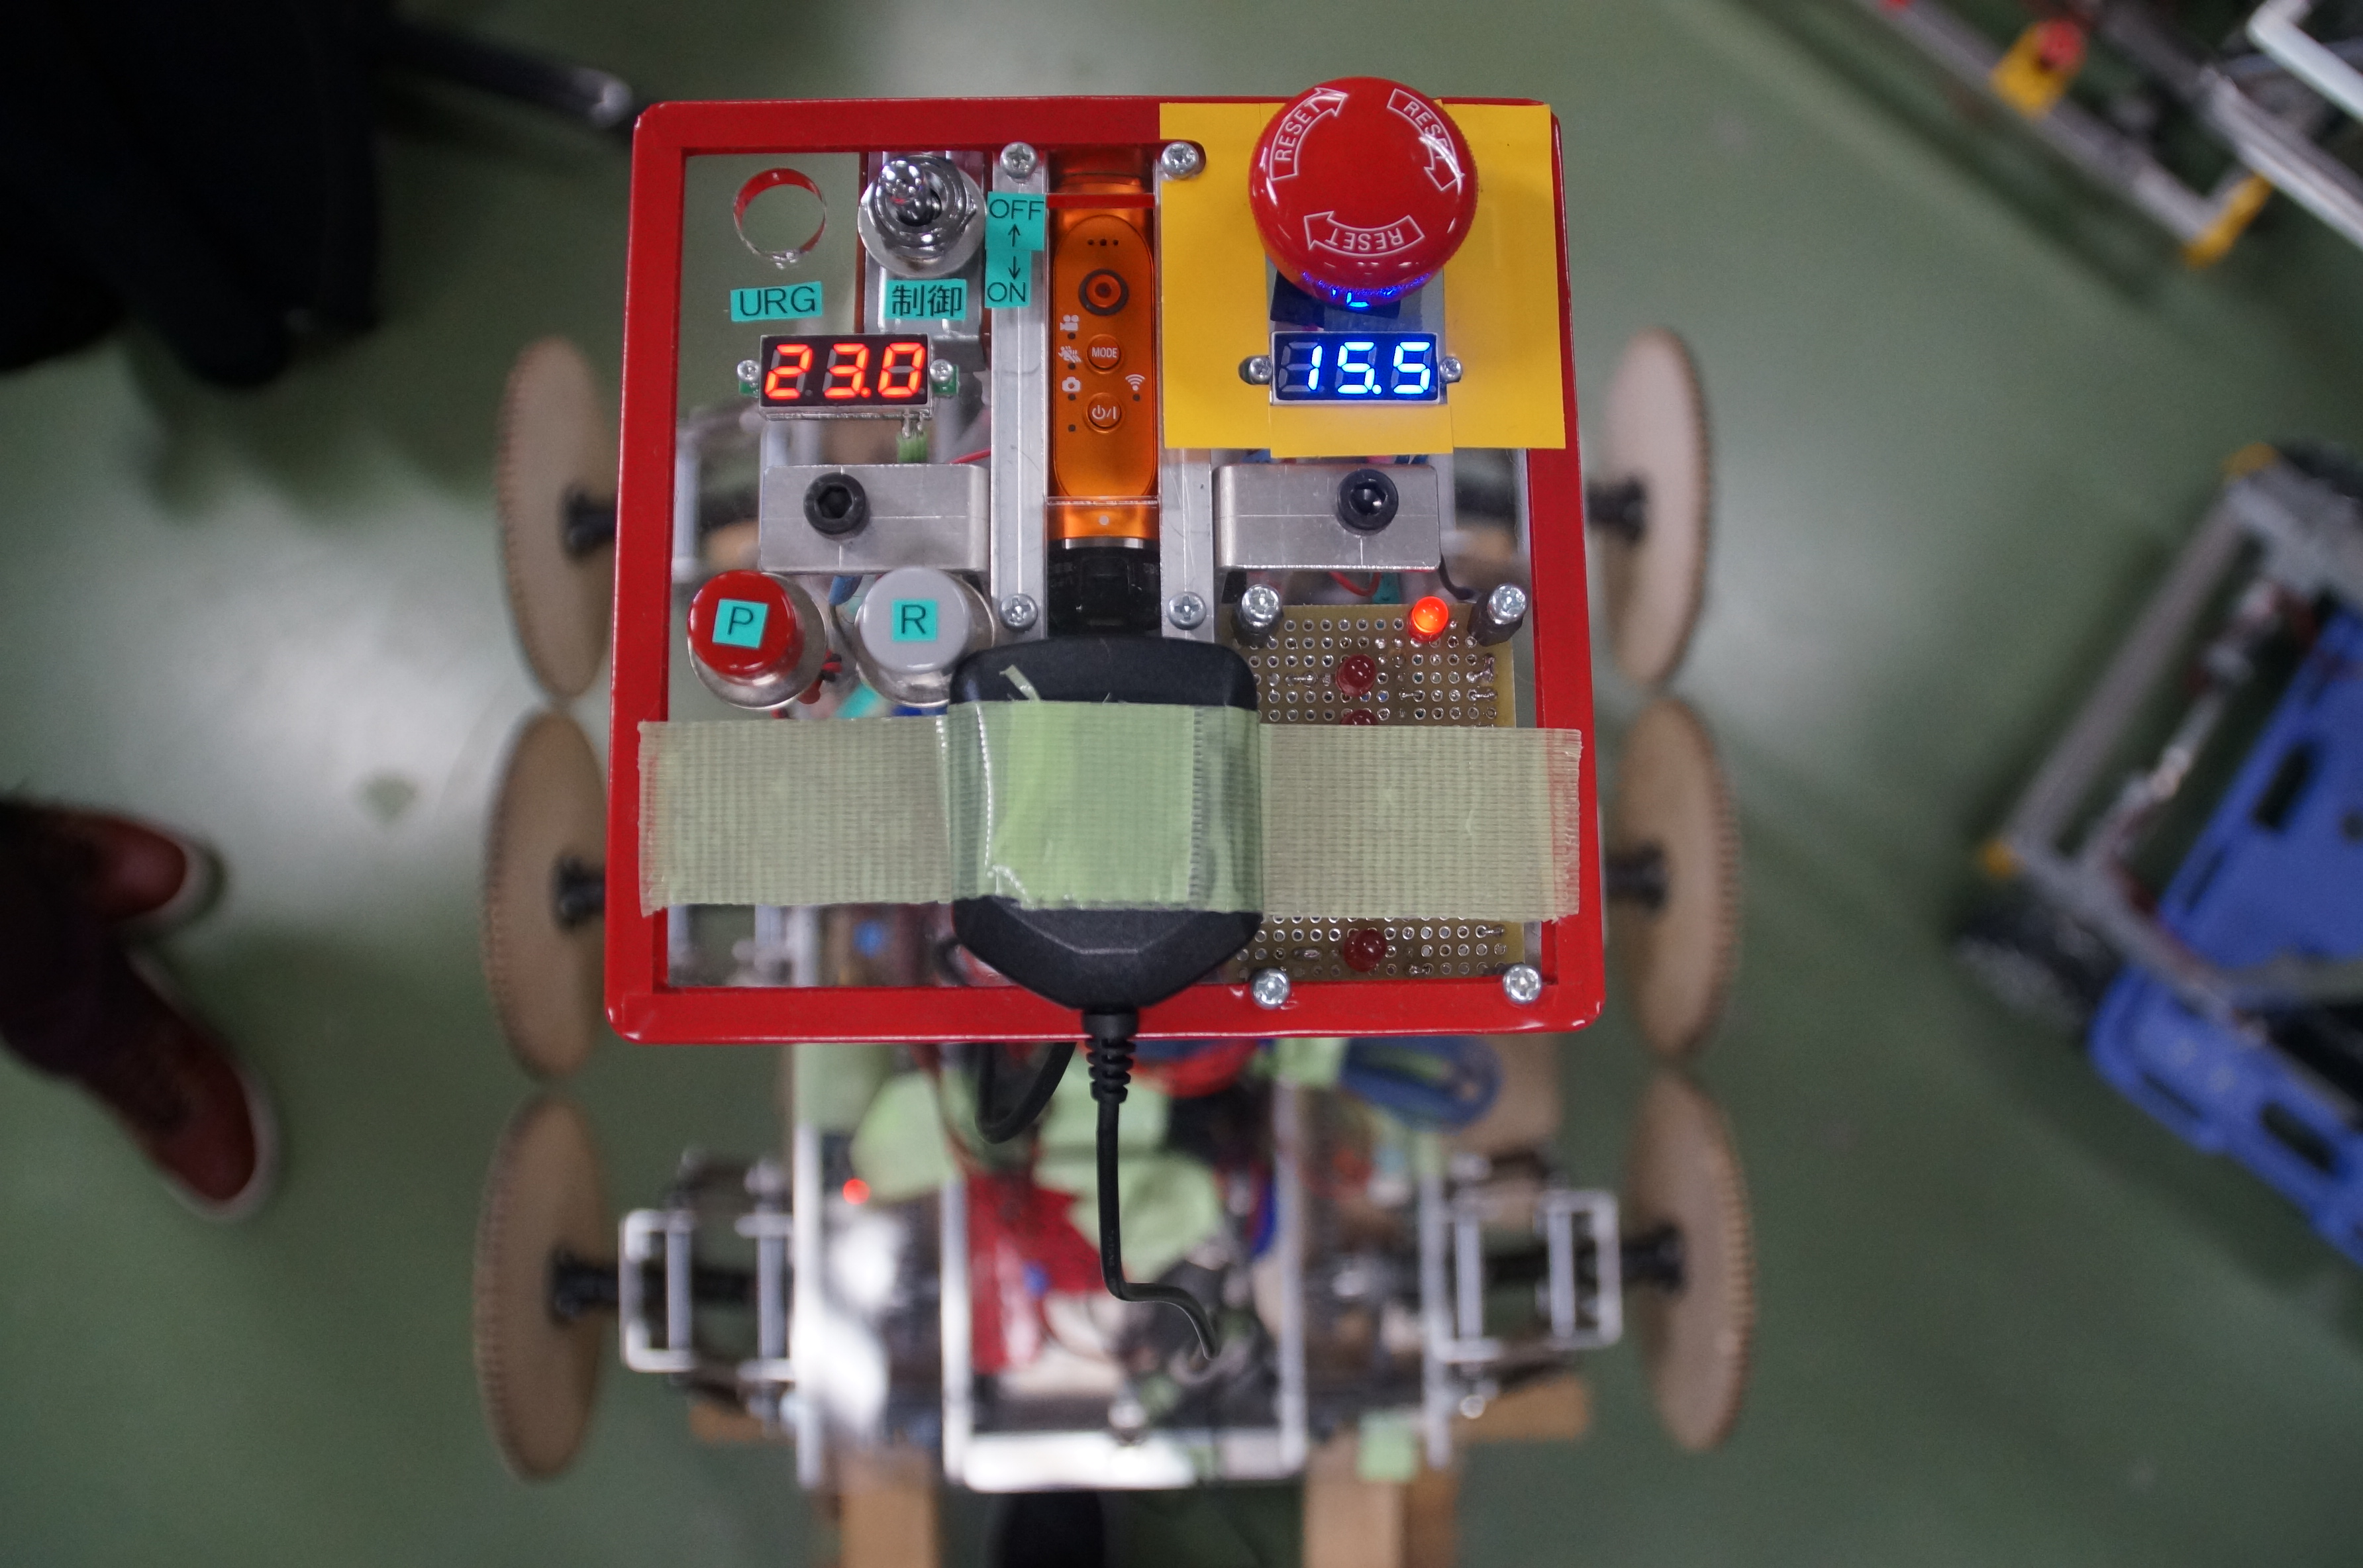
\includegraphics[width=80mm]{img/soft/DSC07946.jpg}
  \caption{操作パネル}
  \label{fig:start_panel}%ここに文章中で使用する名前を指定する
 \end{center}
\end{figure}

\subsection{無線通信}
\begin{enumerate}
\item 使用するデバイスをロボットが接続しているネットワークと同じネットワークに接続する.
\item sshコマンドを用いてロボットとデバイスを接続する.

例 ssh ubuntu@192.168.2.116  ssh ユーザー名@ロボットのIPアドレス   
\item 接続が完了するとデバイス側のユーザー名がロボットのユーザー名に切り替わる.
\item 接続できない場合はロボットがネットワークに接続しているか確認する(ロボットのWi-Fiドングルが機能しているかなど).  
\end{enumerate}

\subsection{Dualshock3のBluetooth接続}
\begin{enumerate}
\item Dualshock3のペアリングが完了している場合,4まで飛ばして良い.
\item 接続したいDualshock3をロボットと有線接続する.
\item ロボットでsixpairを実行する
\item ロボットで以下のコマンドを入力する.
\item sudo hciconfig hci0 piscan
\item sixad -s \&
\item 「sixad started, press the PS button now」と表示されたらDualshock3のPSボタンを長押しする.
\item Dualshock3が振動が収まり,ポートランプの1番が点灯したら接続が完了する.
\end{enumerate}
\subsection{プログラムの実行}
\begin{enumerate}
\item /home/ubuntu/Desktop/TsukubaChallge2016/tsukuba2016に移動する.
\item センサ類が全て接続されているのを確認する.
\item フォルダ内のtsukuba2016を実行する.
\item プログラムは待機モード起動し,□ボタンを押すと手動走行モード,△ボタンを押すと自律走行モードに移行する.
\item 各モードからは×ボタンで待機モードに戻ることができ,待機モードでstartボタンを押すと終了する.
\end{enumerate}
